\documentclass[handout]{ximera}
%\documentclass[10pt,handout,twocolumn,twoside,wordchoicegiven]{xercises}
%\documentclass[10pt,handout,twocolumn,twoside,wordchoicegiven]{xourse}

%\author{Steven Gubkin}
%\license{Creative Commons 3.0 By-NC}
%\usepackage{todonotes}

\newcommand{\todo}{}

\usepackage{esint} % for \oiint
\graphicspath{
{./}
{functionsOfSeveralVariables/}
{normalVectors/}
{lagrangeMultipliers/}
{vectorFields/}
{greensTheorem/}
{shapeOfThingsToCome/}
}


\usepackage{tkz-euclide}
\tikzset{>=stealth} %% cool arrow head
\tikzset{shorten <>/.style={ shorten >=#1, shorten <=#1 } } %% allows shorter vectors

\usetikzlibrary{backgrounds} %% for boxes around graphs
\usetikzlibrary{shapes,positioning}  %% Clouds and stars
\usetikzlibrary{matrix} %% for matrix
\usepgfplotslibrary{polar} %% for polar plots
\usetkzobj{all}
\usepackage[makeroom]{cancel} %% for strike outs
%\usepackage{mathtools} %% for pretty underbrace % Breaks Ximera
\usepackage{multicol}
\usepackage{pgffor} %% required for integral for loops


%% http://tex.stackexchange.com/questions/66490/drawing-a-tikz-arc-specifying-the-center
%% Draws beach ball
\tikzset{pics/carc/.style args={#1:#2:#3}{code={\draw[pic actions] (#1:#3) arc(#1:#2:#3);}}}



\usepackage{array}
\setlength{\extrarowheight}{+.1cm}   
\newdimen\digitwidth
\settowidth\digitwidth{9}
\def\divrule#1#2{
\noalign{\moveright#1\digitwidth
\vbox{\hrule width#2\digitwidth}}}





\newcommand{\RR}{\mathbb R}
\newcommand{\R}{\mathbb R}
\newcommand{\N}{\mathbb N}
\newcommand{\Z}{\mathbb Z}

%\newcommand{\sage}{\textsf{SageMath}}


%\renewcommand{\d}{\,d\!}
\renewcommand{\d}{\mathop{}\!d}
\newcommand{\dd}[2][]{\frac{\d #1}{\d #2}}
\newcommand{\pp}[2][]{\frac{\partial #1}{\partial #2}}
\renewcommand{\l}{\ell}
\newcommand{\ddx}{\frac{d}{\d x}}

\newcommand{\zeroOverZero}{\ensuremath{\boldsymbol{\tfrac{0}{0}}}}
\newcommand{\inftyOverInfty}{\ensuremath{\boldsymbol{\tfrac{\infty}{\infty}}}}
\newcommand{\zeroOverInfty}{\ensuremath{\boldsymbol{\tfrac{0}{\infty}}}}
\newcommand{\zeroTimesInfty}{\ensuremath{\small\boldsymbol{0\cdot \infty}}}
\newcommand{\inftyMinusInfty}{\ensuremath{\small\boldsymbol{\infty - \infty}}}
\newcommand{\oneToInfty}{\ensuremath{\boldsymbol{1^\infty}}}
\newcommand{\zeroToZero}{\ensuremath{\boldsymbol{0^0}}}
\newcommand{\inftyToZero}{\ensuremath{\boldsymbol{\infty^0}}}



\newcommand{\numOverZero}{\ensuremath{\boldsymbol{\tfrac{\#}{0}}}}
\newcommand{\dfn}{\textbf}
%\newcommand{\unit}{\,\mathrm}
\newcommand{\unit}{\mathop{}\!\mathrm}
\newcommand{\eval}[1]{\bigg[ #1 \bigg]}
\newcommand{\seq}[1]{\left( #1 \right)}
\renewcommand{\epsilon}{\varepsilon}
\renewcommand{\phi}{\varphi}


\renewcommand{\iff}{\Leftrightarrow}

\DeclareMathOperator{\arccot}{arccot}
\DeclareMathOperator{\arcsec}{arcsec}
\DeclareMathOperator{\arccsc}{arccsc}
\DeclareMathOperator{\si}{Si}
\DeclareMathOperator{\proj}{\vec{proj}}
\DeclareMathOperator{\scal}{scal}
\DeclareMathOperator{\sign}{sign}


%% \newcommand{\tightoverset}[2]{% for arrow vec
%%   \mathop{#2}\limits^{\vbox to -.5ex{\kern-0.75ex\hbox{$#1$}\vss}}}
\newcommand{\arrowvec}{\overrightarrow}
%\renewcommand{\vec}[1]{\arrowvec{\mathbf{#1}}}
\renewcommand{\vec}{\mathbf}
\newcommand{\veci}{{\boldsymbol{\hat{\imath}}}}
\newcommand{\vecj}{{\boldsymbol{\hat{\jmath}}}}
\newcommand{\veck}{{\boldsymbol{\hat{k}}}}
\newcommand{\vecl}{\boldsymbol{\l}}
\newcommand{\uvec}[1]{\mathbf{\hat{#1}}}
\newcommand{\utan}{\mathbf{\hat{t}}}
\newcommand{\unormal}{\mathbf{\hat{n}}}
\newcommand{\ubinormal}{\mathbf{\hat{b}}}

\newcommand{\dotp}{\bullet}
\newcommand{\cross}{\boldsymbol\times}
\newcommand{\grad}{\boldsymbol\nabla}
\newcommand{\divergence}{\grad\dotp}
\newcommand{\curl}{\grad\cross}
%\DeclareMathOperator{\divergence}{divergence}
%\DeclareMathOperator{\curl}[1]{\grad\cross #1}
\newcommand{\lto}{\mathop{\longrightarrow\,}\limits}

\renewcommand{\bar}{\overline}

\colorlet{textColor}{black} 
\colorlet{background}{white}
\colorlet{penColor}{blue!50!black} % Color of a curve in a plot
\colorlet{penColor2}{red!50!black}% Color of a curve in a plot
\colorlet{penColor3}{red!50!blue} % Color of a curve in a plot
\colorlet{penColor4}{green!50!black} % Color of a curve in a plot
\colorlet{penColor5}{orange!80!black} % Color of a curve in a plot
\colorlet{penColor6}{yellow!70!black} % Color of a curve in a plot
\colorlet{fill1}{penColor!20} % Color of fill in a plot
\colorlet{fill2}{penColor2!20} % Color of fill in a plot
\colorlet{fillp}{fill1} % Color of positive area
\colorlet{filln}{penColor2!20} % Color of negative area
\colorlet{fill3}{penColor3!20} % Fill
\colorlet{fill4}{penColor4!20} % Fill
\colorlet{fill5}{penColor5!20} % Fill
\colorlet{gridColor}{gray!50} % Color of grid in a plot

\newcommand{\surfaceColor}{violet}
\newcommand{\surfaceColorTwo}{redyellow}
\newcommand{\sliceColor}{greenyellow}




\pgfmathdeclarefunction{gauss}{2}{% gives gaussian
  \pgfmathparse{1/(#2*sqrt(2*pi))*exp(-((x-#1)^2)/(2*#2^2))}%
}


%%%%%%%%%%%%%
%% Vectors
%%%%%%%%%%%%%

%% Simple horiz vectors
\renewcommand{\vector}[1]{\left\langle #1\right\rangle}


%% %% Complex Horiz Vectors with angle brackets
%% \makeatletter
%% \renewcommand{\vector}[2][ , ]{\left\langle%
%%   \def\nextitem{\def\nextitem{#1}}%
%%   \@for \el:=#2\do{\nextitem\el}\right\rangle%
%% }
%% \makeatother

%% %% Vertical Vectors
%% \def\vector#1{\begin{bmatrix}\vecListA#1,,\end{bmatrix}}
%% \def\vecListA#1,{\if,#1,\else #1\cr \expandafter \vecListA \fi}

%%%%%%%%%%%%%
%% End of vectors
%%%%%%%%%%%%%

%\newcommand{\fullwidth}{}
%\newcommand{\normalwidth}{}



%% makes a snazzy t-chart for evaluating functions
%\newenvironment{tchart}{\rowcolors{2}{}{background!90!textColor}\array}{\endarray}

%%This is to help with formatting on future title pages.
\newenvironment{sectionOutcomes}{}{} 



%% Flowchart stuff
%\tikzstyle{startstop} = [rectangle, rounded corners, minimum width=3cm, minimum height=1cm,text centered, draw=black]
%\tikzstyle{question} = [rectangle, minimum width=3cm, minimum height=1cm, text centered, draw=black]
%\tikzstyle{decision} = [trapezium, trapezium left angle=70, trapezium right angle=110, minimum width=3cm, minimum height=1cm, text centered, draw=black]
%\tikzstyle{question} = [rectangle, rounded corners, minimum width=3cm, minimum height=1cm,text centered, draw=black]
%\tikzstyle{process} = [rectangle, minimum width=3cm, minimum height=1cm, text centered, draw=black]
%\tikzstyle{decision} = [trapezium, trapezium left angle=70, trapezium right angle=110, minimum width=3cm, minimum height=1cm, text centered, draw=black]

\outcome{Practice Limits.}
   

\title{Limits exercises}

\begin{document}
\begin{abstract}
Here is an opportunity for you to practice limits.
\end{abstract}
\maketitle

\begin{exercise}
  Evaluate the expressions by referencing the graph of $f(x)$ below. Write DNE if the limit or function value does not exist.
  
\begin{center} 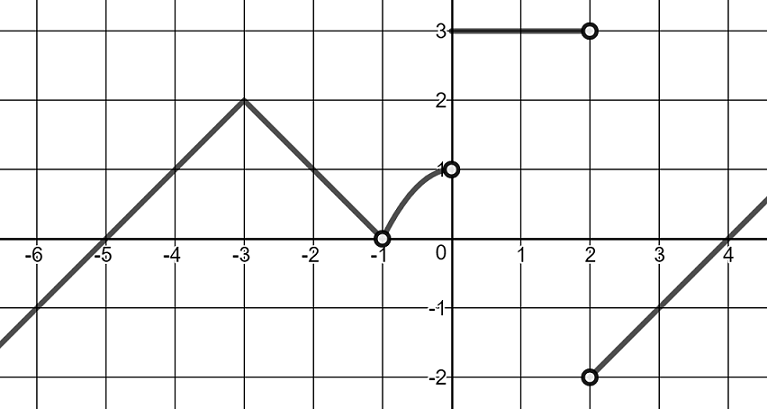
\includegraphics[scale=0.5]{limgraph.png} \end{center}

\begin{enumerate}

\begin{multicols}{3}
\item [] $\displaystyle\lim_{x\to -3^-} f(x) =\answer{2}$  

\item [] $\displaystyle\lim_{x\to -3^+} f(x) = \answer{2}$ 

\item [] $\displaystyle\lim_{x\to -3} f(x) = \answer{2}$ 

\item [] $f(-3) = \answer{2}$

\item [] $\displaystyle\lim_{x\to -1^-} f(x) =\answer{0}$ 

\item [] $\displaystyle\lim_{x\to -1^+} f(x) = \answer{0}$ 

\item [] $\displaystyle\lim_{x\to -1} f(x) = \answer{0}$ 

\item [] $f(-1) = \answer{DNE}$

\item [] $\displaystyle\lim_{x\to 0^-} f(x) =\answer{1}$ 

\item [] $\displaystyle\lim_{x\to 0^+} f(x) = \answer{3}$ 

\item [] $\displaystyle\lim_{x\to 0} f(x) = \answer{DNE}$ 

\item [] $f(0) = \answer{3}$

\item [] $\displaystyle\lim_{x\to 2^-} f(x) =\answer{3}$ 

\item [] $\displaystyle\lim_{x\to 2^+} f(x) = \answer{-2}$ 

\item [] $\displaystyle\lim_{x\to 2} f(x) = \answer{DNE}$ 

\item [] $f(2) = \answer{DNE}$

\end{multicols}

\item [] $\displaystyle\lim_{x\to 4} f(x) = \answer{0}$ 

\end{enumerate}

\end{exercise}

\begin{exercise}

Consider the statement below, and then indicate whether it is sometimes, always, or never true.

\begin{center} ``If $f(10)$ exists, then $\displaystyle\lim_{x\to 10} f(x) = f(10).$" \end{center}

This statement is \wordChoice{\choice[correct]{sometimes}\choice{always}\choice{never}} true.

\begin{hint}

Use the data you gathered in the previous exercise to help you answer this question.  

\end{hint}

\end{exercise}

\begin{exercise}

Consider the statement below, and then indicate whether it is sometimes, always, or never true.

\begin{center} ``If $\displaystyle\lim_{x\to 10^-} f(x) = 4$ and $\displaystyle\lim_{x\to 10} f(x)$ exists, then $\displaystyle\lim_{x\to 10^+} f(x) = 4.$" \end{center}

This statement is \wordChoice{\choice{sometimes}\choice[correct]{always}\choice{never}} true.

\begin{hint}

Use the data you gathered in the first exercise to help you answer this question.  You may also want to review how one-sided and two-sided limits relate to one another using the  \href{https://ximera.osu.edu/math160fa17/m160exam1content/whatIsALimit/digInWhatIsALimit}{previous card}.
\end{hint}

\end{exercise}

\begin{exercise}

Consider the statement below, and then indicate whether it is sometimes, always, or never true.

\begin{center} ``If $\displaystyle\lim_{x\to 10^-} f(x) = \displaystyle\lim_{x\to 10^+} f(x)$, then $\displaystyle\lim_{x\to 10} f(x)$ may not exist." \end{center}

This statement is \wordChoice{\choice{sometimes}\choice{always}\choice[correct]{never}} true.

\begin{hint}

Use the data you gathered in the first exercise to help you answer this question.  You may also want to review how one-sided and two-sided limits relate to one another using the \href{https://ximera.osu.edu/math160fa17/m160exam1content/whatIsALimit/digInWhatIsALimit}{previous card}.

\end{hint} 

\end{exercise}

\begin{exercise}
Use $f(x) = x^2$ to fill in the table below.
  \[
  \begin{array}{l|l}
    x      & f(x)      \\ \hline
    1.1    & \begin{prompt}\answer{1.21}\end{prompt}\\
    1.01   & \begin{prompt}\answer{1.0201}\end{prompt}\\
    1.001  & \begin{prompt}\answer{1.002001}\end{prompt}\\
    1.0001 & \begin{prompt}\answer{1.00020001}\end{prompt}\\
    1.00001 & \begin{prompt}\answer{1.00020001}\end{prompt}\\
    1.000001 & \begin{prompt}\answer{1.0000200001}\end{prompt}
  \end{array}
  \]
  Based on the data you have gathered, you would predict that 
  \[
  \lim_{x\to 1} x^2 = \answer{1}
  \]
  
    \begin{exercise}
    As discussed previously, neither tables nor graphs can ever tell you for certain what a limit is equal to. However, sometimes they can help to ``guess'' the limit. Let's look at the graph of $f(x) = x^2$ to double check your prediction. 
\[
\graph{x^2}
\]

Does the graph of $f(x) = x^2$ support your previous prediction that $\lim_{x\to 1} x^2 = 1$? 

\begin{multipleChoice}
    \choice[correct]{Yes}
    \choice{No}
    
\begin{feedback}[correct]

In this case, the fact that $\lim_{x\to 1} x^2 = 1$ is evident from the above table and from the graph of $f(x) = x^2$.  In the next section, you will learn how to calculate that $\lim_{x\to 1} x^2 = 1$ without having to rely on tables and graphs.  In the meantime, your main tool to evaluate limits will be to use graphs or tables, but make sure to be extra careful when doing so: tables and graphs can be misleading! 

\end{feedback}
\end{multipleChoice}
    \end{exercise}

\end{exercise}

\begin{exercise}
Use $g(x) = \cos\left(\frac{\pi}{x-2\pi}\right)$ to fill in the table below.
  \[
  \begin{array}{l|l}
    x      & f(x)      \\ \hline
    2\pi + 0.1    & \begin{prompt}\answer{1}\end{prompt}\\
    2\pi + 0.01    & \begin{prompt}\answer{1}\end{prompt}\\
    2\pi + 0.001   & \begin{prompt}\answer{1}\end{prompt}\\
    2\pi + 0.0001  & \begin{prompt}\answer{1}\end{prompt}\\
    2\pi + 0.00001 & \begin{prompt}\answer{1}\end{prompt}
  \end{array}
  \]
  Based on the data you have gathered, you would predict that 
  \[
  \lim_{x\to 2\pi}  \cos\left(\frac{\pi}{x-2\pi}\right)= \answer{1}
  \]
  
    \begin{exercise}
Let's look at the graph of $g(x) = \cos\left(\frac{\pi}{x-2\pi}\right)$ to double check your prediction. 
\[
\graph{\cos\left(\frac{\pi}{x-2\pi}\right)}
\]

Does the graph of $g(x) = \cos\left(\frac{\pi}{x-2\pi}\right)$ support your previous prediction that $\lim_{x\to 1} \cos\left(\frac{\pi}{x-2\pi}\right) = 1$? 

\begin{multipleChoice}
    \choice{Yes}
    \choice[correct]{No}
    
\begin{feedback}[correct]

Even though the table you filled out seems to indicate that $\lim_{x\to 2\pi}  \cos\left(\frac{\pi}{x-2\pi}\right)= 1$, it turns out that this limit actually does not exist, as the graph of $g(x)$ shows.  This is yet another example of why tables are not a fool-proof method for evaluating limits.  Case in point: be very careful when using tables to make conclusions about limits! 

\end{feedback}
\end{multipleChoice}
    \end{exercise}

\end{exercise}

\end{document}
